\section{OctoTentacle}
\paragraph{}
La partie OctoTentacle de notre logiciel est le côté client. C'est un module qui est installé sur un hôte afin de pouvoir être superviser et auditer par le serveur.

\subsection{Algorithme}
\paragraph{}
Le client est divisé en deux parties principales : une partie pour l'enregistrement du client auprès du serveur et une partie qui permet d'interagir avec le serveur pour l'éxécution des scripts et l'envoi des rapports.

\begin{figure}[!h]
    \begin{center}
        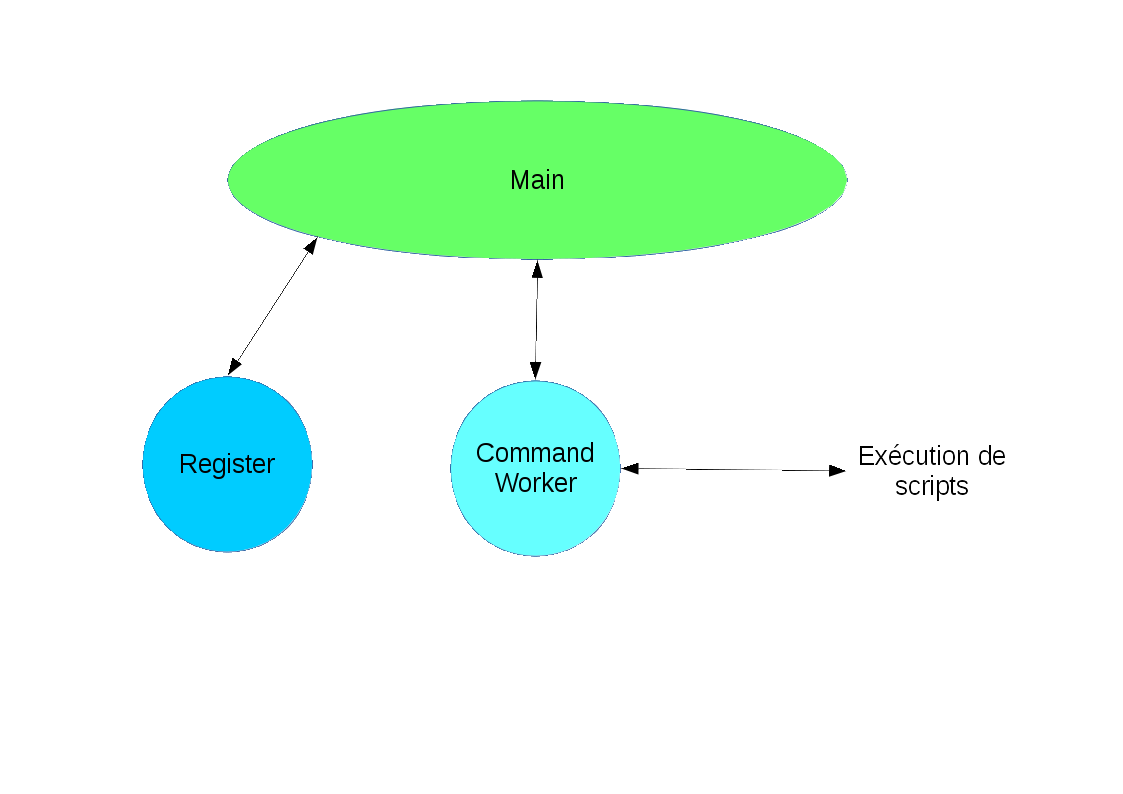
\includegraphics[width=1\textwidth]{img/algo_tentacle.png}
        \caption{Fonctionnement technique du Tentacle}
    \end{center} 
\end{figure}

\subsection{Register}
\paragraph{}
La partie enregistrement du client possède deux fonctions : une première fonction qui est un daemon et attend qu'un serveur d'administration le contacte pour proposer un enregistrement sur le réseau, une seconde fonction qui est à l'initiative de l'enregistrement auprès du brain en connaissant son adresse IP. 
Le daemon d'enregistrement écoute sur le port 7000. Lorsqu'un serveur souhaite enregistrer le client sur son réseau, il y a un échange d'informations. Le client donne son hostname, le serveur lui fournit  un ID et une clé générée par le brain et qui permettra de sécuriser l'authentification entre le client et le serveur. Une fois l'enregistrement terminé, le thread se termine et un nouveau thread se lance, le daemon de scripts.
Si lors de son lancement le client a en paramètre l'adresse IP d'un serveur avec l'option -b, le client va alors contacter directement le serveur pour demander à être enregistrer. L'enregistrement se fait ensuite de la même manière.

\subsection{CommandWorker}
\paragraph{}
Le CommandWorker est un processus du Tentacle qui permet la réception des demandes d'éxécution de script de la part du Brain, l'éxécution de ces commandes et l'envoi des résultats vers le Brain.
\paragraph{}
Dans un premier temps, le Tentacle se place en écoute sur le port 7001. Quand le Brain auquel il est affilié se connecte sur ce socket, il y a authentification des parties et le Brain demande au Tentacle d'éxécuter un script qu'il possède. 
La connexion se ferme ensuite. Le Tentacle éxécute alors le script demandé en local et sauvegarde le retour du script dans un fichier en local. 
Une fois le fichier sauvegardé en local, le Tentacle va initier une connexion avec le Brain sur le port 6001 en demandant la sauvegarde du résultat du script en base de données.
Le contenu du fichier est donc envoyé au Brain et le résultat sera ensuite accessible pour l'administrateur via l'interface Web.